\chapter{Elliptic Curve Cryptography}
\label{chap:elliptic}

We now begin our discussion of \gls{ecc};
that is, cryptography which uses \glspl{elliptic curve}.
In this chapter we focus on a variant of the \gls{dhke}
which uses a \gls{cyclic group} based on \glspl{elliptic curve}.
We also present \glspl{signature} based on \glspl{elliptic curve}
which are generalizations of Schnorr signatures and DSA.



\section{Problems with Subgroups of Finite Fields}
\label{sec:Fp_problems}

One of the difficulties with $\F_{p}^{*}$
is that each prime $p$ uniquely determines the potential
multiplicative \glspl{subgroup}.
The security depends on the factorization of $p-1$;
this factorization will determine how difficult it is to solve
the \gls{dlp}, which is the basis for security.
Additionally, there are subexponential algorithms which can solve
the \gls{dlp} over $\F_{p}$;
a brief discussion of the \emph{index calculus algorithm}
may be found in \cite[Chapter~10.3]{IntroModernCrypto}.
These facts imply that the size of $p$ must be chosen quite large;
see Chapter~\ref{chap:hardness} and Table~\ref{table:key_lengths}
for more information.
Large values of $p$ implies greater computational and storage costs.
This makes them challenging to use in resource-constrained environments.

\Glspl{elliptic curve} solve this problem.
For any given prime $p$, there are many \glspl{elliptic curve}
which can be defined over the \gls{finite field} $\F_{p}$.
We have $\#E(\F_{p})\simeq p$;
see Theorem~\ref{thm:hasse_bound} for a more information.
Given the freedom of both the underlying \gls{finite field}
and the \gls{elliptic curve} equation,
it would seem reasonable that certain \glspl{elliptic curve} could be
constructed with desirable properties;
this is the case.
Furthermore, there are large classes of \glspl{elliptic curve}
where the best known algorithms for solving the \gls{dlp} are \emph{generic};
that is, the methods work on all \glspl{group} and do not take advantage
of the algebraic structure of the \gls{elliptic curve}.

For 128-bit security, it is suggested that $p$ be a 3072-bit prime
for DSA and DH performed inside \glspl{subgroup} of $\F_{p}^{*}$.
Storing a 3072-bit public key requires 384 bytes.
This is significant storage requirement.
A similar security level requires
an \gls{elliptic curve} over a 256-bit prime \gls{field};
the public key is 64 bytes (uncompressed).
As mentioned before, see the discussion in Chapter~\ref{chap:hardness}
and Table~\ref{table:key_lengths}.
Of course, the smaller size of public key requires more complicated
group arithmetic, and care must be taken that these
methods are computed securely.



\section{Elliptic Curve Diffie-Hellman (ECDH)}
\label{sec:ecdh}

\subsection{Discussion}

Elliptic Curve Diffie-Hellman (ECDH) is the \gls{dhke} over
\glspl{group} based on \glspl{elliptic curve}.
The definition is exactly the same as
Def.~\ref{def:diffie-hellman}
in Chapter~\ref{sec:public_diffie_hellman};
the only difference is that we are using a different \gls{cyclic group}.

\subsection{Examples}

Plots for Examples~\ref{example:ecc_ecdh_1} and \ref{example:ecc_ecdh_2}
may be found in Figure~\ref{fig:ec_finite_plots_ecdh}.

\begin{figure}[p]
\centering
    \begin{subfigure}[t]{\textwidth}
        \centering
    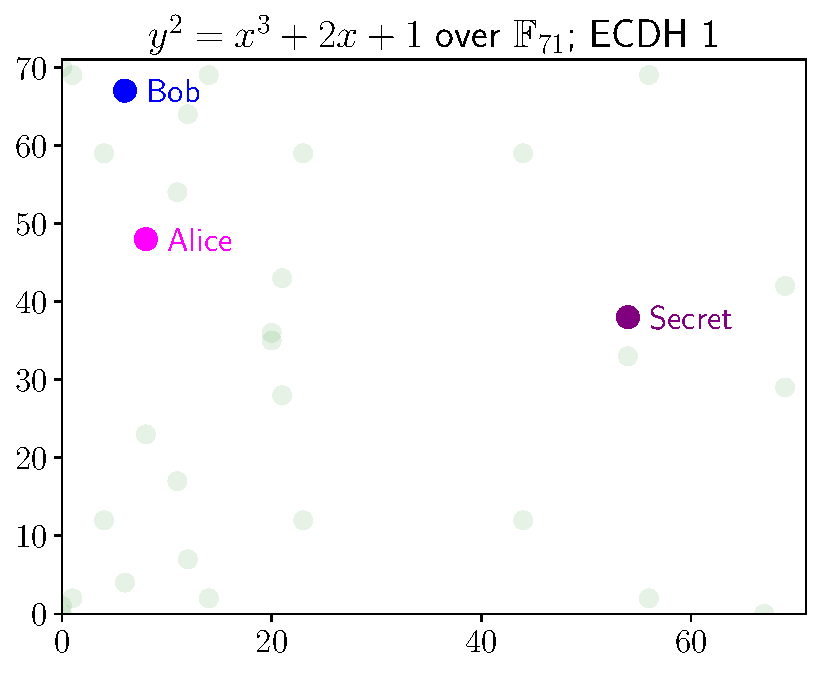
\includegraphics[width=0.70\textwidth]{plots/ec_finite/ec_finite_F_71_2_1_ecdh_1.pdf}
    \caption{Plot of Alice's public key ${\color{magenta}{A}} = \parens{8,48}$,
    Bob's public key ${\color{blue}{B}} = \parens{6,67}$,
    and the \gls{shared secret} ${\color{purple}{K}} = \parens{54,38}$
    for Example~\ref{example:ecc_ecdh_1}.}
    \label{fig:ec_finite_plots_ecdh_1}
    \end{subfigure}

    \begin{subfigure}[t]{\textwidth}
        \centering
    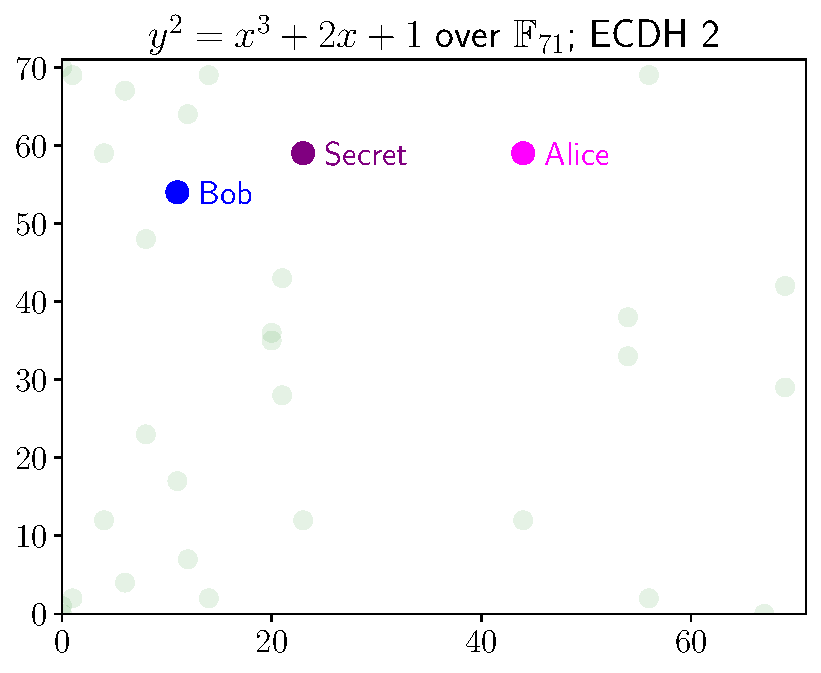
\includegraphics[width=0.70\textwidth]{plots/ec_finite/ec_finite_F_71_2_1_ecdh_2.pdf}
    \caption{Plot of Alice's public key ${\color{magenta}{A}} = \parens{44,59}$,
    Bob's public key ${\color{blue}{B}} = \parens{11,54}$,
    and the \gls{shared secret} ${\color{purple}{K}} = \parens{23,59}$
    for Example~\ref{example:ecc_ecdh_2}.}
    \label{fig:ec_finite_plots_ecdh_2}
    \end{subfigure}

\caption[Plots of public keys and shared secrets for ECDH]{Here
    we plot Alice's public key ${\color{magenta}{A}} = a\cdot P$,
    Bob's public key ${\color{blue}{B}} = b\cdot P$,
    and the \gls{shared secret} ${\color{purple}{K}} = (ab)\cdot P$
    for Examples~\ref{example:ecc_ecdh_1} and \ref{example:ecc_ecdh_2}.
    }
\label{fig:ec_finite_plots_ecdh}
\end{figure}


\begin{example}[Elliptic Curve Diffie-Hellman 1]
\label{example:ecc_ecdh_1}
\exampleCodeReference{examples/ecc/ecdh\_1.py}

We continue with the \gls{elliptic curve}

\begin{equation}
    E: y^{2} = x^{3} + 2x + 1
\end{equation}

\noindent
over $\F_{71}$.
This curve was previously used in Chapter~\ref{sec:math_elliptic_curves}.
We will use this curve along with the base point $P=\parens{0,1}$.
We can see that $\abs{\angles{\parens{0,1}}}=32$;
that is, the point $\parens{0,1}$ generates a \gls{subgroup} of order 32.

Alice chooses her private key so that

\begin{align}
    a &= 29 \nonumber\\
    A &= a\cdot P \nonumber\\
        &= 29\cdot\parens{0,1} \nonumber\\
        &= \parens{8,48}.
\end{align}

\noindent
Similarly, Bob chooses his private key so that

\begin{align}
    b &= 14 \nonumber\\
    B &= b\cdot P \nonumber\\
        &= 14\cdot\parens{0,1} \nonumber\\
        &= \parens{6,67}.
\end{align}

Alice retrieves Bob's public key and computes

\begin{align}
    K &= a\cdot B \nonumber\\
        &= 29\cdot\parens{6,67} \nonumber\\
        &= \parens{54,38}.
\end{align}

\noindent
Bob learns Alice's public key and determines

\begin{align}
    K &= b\cdot A \nonumber\\
        &= 14\cdot\parens{8,48} \nonumber\\
        &= \parens{54,38}.
\end{align}

\noindent
They can now use this \gls{shared secret} to derive a secret key
for secure communication.
See Figure~\ref{fig:ec_finite_plots_ecdh_1} for a plot of

\begin{align}
    \color{magenta}{A} &\mathbin{\color{magenta}{=}}
        \color{magenta}{\parens{8,48}} \nonumber\\
    \color{blue}{B} &\mathbin{\color{blue}{=}}
        \color{blue}{\parens{6,67}} \nonumber\\
    \color{purple}{K} &\mathbin{\color{purple}{=}}
        \color{purple}{\parens{54,38}}.
\end{align}
\end{example}

\begin{example}[Elliptic Curve Diffie-Hellman 2]
\label{example:ecc_ecdh_2}
\exampleCodeReference{examples/ecc/ecdh\_2.py}

We continue with the setup we used in Example~\ref{example:ecc_ecdh_1}
with the \gls{elliptic curve}

\begin{equation}
    E: y^{2} = x^{3} + 2x + 1
\end{equation}

\noindent
over $\F_{71}$ and base point $P = \parens{0,1}$.
The order of the \gls{group} is 32.

Alice chooses

\begin{align}
    a &= 17 \nonumber\\
    A &= a\cdot P \nonumber\\
        &= 17\cdot\parens{0,1} \nonumber\\
        &= \parens{44,59}
\end{align}

\noindent
while Bob chooses

\begin{align}
    b &= 27 \nonumber\\
    B &= b\cdot P \nonumber\\
        &= 27\cdot\parens{0,1} \nonumber\\
        &= \parens{11,54}.
\end{align}

Alice retrieves Bob's public key and computes

\begin{align}
    K &= a\cdot B \nonumber\\
        &= 17\cdot\parens{11,54} \nonumber\\
        &= \parens{23,59}.
\end{align}

\noindent
Bob learns Alice's public key and determines

\begin{align}
    K &= b\cdot A \nonumber\\
        &= 27\cdot\parens{44,59} \nonumber\\
        &= \parens{23,59}.
\end{align}

\noindent
They can now use this \gls{shared secret} to derive a secret key
for secure communication.
See Figure~\ref{fig:ec_finite_plots_ecdh_2} for a plot of

\begin{align}
    \color{magenta}{A} &\mathbin{\color{magenta}{=}}
        \color{magenta}{\parens{44, 59}} \nonumber\\
    \color{blue}{B} &\mathbin{\color{blue}{=}}
        \color{blue}{\parens{11,54}} \nonumber\\
    \color{purple}{K} &\mathbin{\color{purple}{=}}
        \color{purple}{\parens{23,59}}.
\end{align}
\end{example}



\section{Elliptic Curve DSA (ECDSA)}
\label{sec:ecdsa}

The Elliptic Curve Digital Signature Algorithm (ECDSA)
reformulates DSA (Def.~\ref{def:dsa})
into a digital signature algorithm for \glspl{elliptic curve}.
There are many similarities with some differences
due to different \glspl{group}.

\subsection{Formal Definition}

\begin{defn}
Let $E/\F_{p}$ be an \gls{elliptic curve} with $G\in E(\F_{p})$
a specified base point and generator.
We assume $\#E(\F_{p}) = n$ is prime.
We fix a \gls{hash function} $H:\braces{0,1}^{*}\to\Z_{n}$.

\paragraph{Key Generation}
Choose private key $d\chooseRandom{}\Z_{n}^{*}$.
The public key is $Q = d\cdot G$.

\paragraph{Signature Generation}
We let $m$ be the message to be signed.
Choose a \gls{nonce} $k\chooseRandom{}\Z_{n}^{*}$.
Set

\begin{align}
    \parens{x,y} &= k\cdot G
        \nonumber\\
    r &= x \mod n
        \nonumber\\
    s &= k^{-1}\brackets{H(m) + rd} \mod n.
\end{align}

\noindent
If $r = 0$, choose another $k$ and repeat.
If $s = 0$, choose another $k$ and repeat.
The signature is $\parens{r,s}$.

\paragraph{Signature Verification}
We receive a signature $\parens{r,s}$ from $Q$ for message $m$.
First, confirm $0 < r < n$, $0 < s < n$, and $n\cdot Q = \mathcal{O}$.
Set

\begin{align}
    w &= s^{-1} \mod n
        \nonumber\\
    u_{1} &= H(m)w \mod n
        \nonumber\\
    u_{2} &= rw \mod n
        \nonumber\\
    \parens{x,y} &= u_{1}\cdot G + u_{2}\cdot Q.
\end{align}

\noindent
The signature is valid if $r = x \mod n$.
\end{defn}

\subsection{Verification}

Let $\parens{r,s}$ be as previously defined for the signature
for message $m$ and public key $Q$.
Then we see

\begin{align}
    \parens{x,y} &= u_{1}\cdot G + u_{2}\cdot Q
            \nonumber\\
        &= \parens{H(m)s^{-1}}\cdot G + \parens{drs^{-1}}\cdot G
            \nonumber\\
        &= s^{-1}\brackets{H(m) + dr}\cdot G
            \nonumber\\
        &= k\cdot G.
    \label{eq:ecc_ecdsa_verify}
\end{align}

\noindent
Thus, we have a valid signature.

\subsubsection{The Necessary Requirement of $r\ne0$}
If $r = 0$, the signature will be valid for any public key.
This should not happen.

\subsubsection{The Necessary Requirement of $s\ne0$}
If $s = 0$, then we cannot compute the modular inverse during
signature verification.
Thus, we cannot verify the signature.

\subsubsection{Nonce Reuse}
Reusing the \gls{nonce} $k$ leads to recovery of the private key.
The reader should work out the details.

\subsection{ECDSA Malleability}
\label{ssec:ecdsa_malleability}

We note that there is some malleability to the signature.
We mean this:
let $\parens{r,s}$ be the signature of message $m$ for public key $Q$.
As noted previously in Eq.~\eqref{eq:ecc_ecdsa_verify},
we have

\begin{align}
    \parens{x,y} &= u_{1}\cdot G + u_{2}\cdot Q \nonumber\\
    r &= x \mod n.
\end{align}

We now look at the pair $\parens{r,-s}$.
In this case, we see

\begin{align}
    \tilde{w} &= \parens{-s}^{-1} \mod n
            \nonumber\\
        &= -w \nonumber\\
    \tilde{u}_{1} &= H(m)w \mod n
            \nonumber\\
        &= -u_{1} \nonumber\\
    \tilde{u}_{2} &= rw \mod n
            \nonumber\\
        &= -u_{2}.
\end{align}

\noindent
This implies that

\begin{align}
    \tilde{u}_{1}\cdot G + \tilde{u}_{2}\cdot Q
            &= -u_{1}\cdot G - u_{2}\cdot Q
        \nonumber\\
    &= -\brackets{u_{1}\cdot G + u_{2}\cdot Q}
        \nonumber\\
    &= -\parens{x,y} \nonumber\\
    &= \parens{x,-y}.
\end{align}

\noindent
Thus, $\parens{r,-s}$ is \emph{also} a valid ECDSA signature 
for message $m$ under the public key $Q$.

While this type of malleability is not of much concern in practice,
we point this out because it will come up when we discuss
Recoverable ECDSA in \gls{ethereum} in
Chapter~\ref{ssec:recoverable_ecdsa_ethereum}.



\section{Problems with ECDSA}

The same problems from biased \glspl{nonce} which arise in DSA
also arise in ECDSA.
Additionally, the nature of scalar multiplication
in \glspl{elliptic curve} requires care to ensure the \gls{nonce} $k$
is not leaked from side-channel analysis
even when using deterministic \glspl{nonce};
we recall that leaking a \gls{nonce} results in the recovery
of the private key.
These side-channel attacks are
\emph{entirely
practical}~\cite{jancar2020minerva,weiser2020big,brumley2011remote}.



\section{Edwards Curve DSA (EdDSA)}

Edwards Curve Digital Signature Algorithm (EdDSA)
was developed to be a digital signature algorithm which would
overcome many of the pitfalls inherent to previous signature algorithms.
In particular, the \gls{nonce} is deterministic in its definition.
Once a private key is computed, there is no further need
for cryptographic random numbers.
This reduces the likelihood of poor implementations.
One of the authors of EdDSA wrote a blog post%
\footnote{\url{https://blog.cr.yp.to/20140323-ecdsa.html}}
about its design;
later, he gave his thoughts%
\footnote{\url{https://blog.cr.yp.to/20191024-eddsa.html}}
on why EdDSA is more immune to attacks than ECDSA.

We do not present a formal definition of EdDSA;
this can be found in references~\cite{ed25519,moreEdDSA,rfc8032}.
The main advantages come from its deterministic nature
(the \gls{nonce} $k$ is deterministic based on the private key and message),
no branch logic (a specific curve type is chosen with \emph{one}
addition formula),
its speed, and the small size of public keys and signatures.
The design helps ensure immunity to side-channel attacks.



\section{Recoverable ECDSA}
\label{sec:recoverable_ecdsa}

In \gls{ethereum}, the ECDSA signatures used are \emph{Recoverable}
ECDSA signatures.
This means that, given the message and associated signature,
it is possible to \emph{recover} the corresponding public key.
The goal of this section to understand this.
First, we work through the process in general before focusing
on the particular case of \gls{ethereum}.

\subsection{Deriving the Public Key from the ECDSA Signature}

We work through the details of deriving the public key from
the message and its ECDSA signature.
We will use the same notation from Chapter~\ref{sec:ecdsa}
and review what we know:

\begin{itemize}
\item \Gls{elliptic curve} $E/\F_{p}$ with generator $G\in E(\F_{p})$.
\item The number of points on the curve $\#E(\F_{p}) = n$ is prime.
\item We have a \gls{hash function} $H:\braces{0,1}^{*}\to\Z_{n}$.
\item We have private key $d\chooseRandom{}\Z_{n}^{*}$ with public key
    $Q = d\cdot G$.
\item We have \gls{nonce} $k\chooseRandom{}\Z_{n}^{*}$.
\item We have a valid signature $\parens{r,s}$ for message $m$ where

\begin{align}
    \parens{x,y} &= k\cdot G \nonumber\\
    r &= x \mod n \nonumber\\
    s &= k^{-1}\brackets{H(m) + rd} \mod n.
\end{align}

A valid signature implies $r\ne0$ and $s\ne0$.
\item We set $P = k\cdot G = \parens{x,y}$.
    The valid signature also implies that

\begin{align}
    w &= s^{-1} \mod n
        \nonumber\\
    u_{1} &= H(m)w \mod n
        \nonumber\\
    u_{2} &= rw \mod n
        \nonumber\\
    P &= u_{1}\cdot G + u_{2}\cdot Q.
\end{align}

This means we can solve for the public key $Q$:

\begin{equation}
    Q = u_{2}^{-1}\brackets{P - u_{1}\cdot G}.
\end{equation}
\end{itemize}

We now walk through the recovery process.
We know that $\parens{x,y} = k\cdot G$, so that $x\in\F_{p}$.
First, we see $r = x \mod n$ so that $r\le x$.
Thus, we have

\begin{equation}
    x = \alpha n + r
    \label{eq:recoverable_ecdsa_x_r}
\end{equation}

\noindent
for $\alpha\ge0$ and $r\in\Z_{n}$.

Previously, we did not make any assumptions about
$n$ and $x$;
we must now make some assumptions in order to proceed.
We either have $p\le n$ or $p > n$.

\begin{itemize}
\item Case 1: $p\le n$

Because we already know $r\le x$, the restriction $p\le n$
implies that $x<n$ so that $x = r$.
This implies that $\alpha=0$ in Eq.~\eqref{eq:recoverable_ecdsa_x_r}.

Now that we have determined $x$, we can find $y$ such that

\begin{equation}
    y^{2} = x^{3} + ax + b.
\end{equation}

\noindent
The points

\begin{align}
    R_{1} &= \parens{x,y} \nonumber\\
    R_{2} &= \parens{x,p-y}
\end{align}

\noindent
are both potential values for $P = k\cdot G$ (assuming $y\ne0$);
because $k$ is unknown, we do not know which is correct.
From here, there are 2 possibilities for the public key $Q$:

\begin{align}
    Q_{1} &= u_{2}^{-1}\brackets{R_{1} - u_{1}\cdot G}
        \nonumber\\
    Q_{2} &= u_{2}^{-1}\brackets{R_{2} - u_{1}\cdot G}.
\end{align}

\noindent
Nothing else can be determined without additional information.

\item Case 2: $p>n$

In this situation, we need to be careful.
Here, we know that $x\ge r$.
From the Hasse Theorem (Theorem~\ref{thm:hasse_bound})
we have $\alpha\in\braces{0,1}$ in Eq.~\eqref{eq:recoverable_ecdsa_x_r}.
This implies we have two possibilities for $x$:
$x_{1} = r$ and $x_{2} = r + n$.
From here, we set $y_{1}$ and $y_{2}$ such that

\begin{align}
    y_{1}^{2} &= x_{1}^{3} + ax_{1} + b
        \nonumber\\
    y_{2}^{2} &= x_{2}^{3} + ax_{2} + b.
\end{align}

\noindent
In this case, there are 4 possible values for $P$:

\begin{align}
    R_{1} &= \parens{x_{1},y_{1}} \nonumber\\
    R_{2} &= \parens{x_{1},p-y_{1}} \nonumber\\
    R_{3} &= \parens{x_{2},y_{2}} \nonumber\\
    R_{4} &= \parens{x_{2},p-y_{2}}.
\end{align}

\noindent
Therefore, there are 4 possibilities for the public key $Q$:

\begin{align}
    Q_{1} &= u_{2}^{-1}\brackets{R_{1} - u_{1}\cdot G}
        \nonumber\\
    Q_{2} &= u_{2}^{-1}\brackets{R_{2} - u_{1}\cdot G}.
        \nonumber\\
    Q_{3} &= u_{2}^{-1}\brackets{R_{3} - u_{1}\cdot G}
        \nonumber\\
    Q_{4} &= u_{2}^{-1}\brackets{R_{4} - u_{1}\cdot G}.
\end{align}

\noindent
Nothing else can be determined without additional information.
\end{itemize}

As noted, additional information is required in order to recover
the specific public key.
For instance, it is sufficient to specify which $x$ value (corresponding
to $\alpha=0$ or $\alpha=1$)
as well as the parity of $y$ (whether $y$ is even or odd).


\subsection{Recoverable ECDSA in Ethereum}
\label{ssec:recoverable_ecdsa_ethereum}

We now walk through Recoverable ECDSA in \gls{ethereum}.

We review material from the
Ethereum Yellowpaper~\cite[Appendix F]{EthereumYellowpaper}.
Note that the paper has been updated and we are referencing
the \emph{Berlin} version;
this is important because different versions use different conventions.

First, we note some differences with the Recoverable ECDSA from above:
instead of the pair $\parens{r,s}$, we have the triple $\parens{r,s,v}$.
Here, we have the restrictions

\begin{align}
    r &\in \braces{1,2,\cdots, n-1} \nonumber\\
    s &\in \braces{1,2,\cdots, \frac{n+1}{2}} \nonumber\\
    v &\in \braces{0,1}.
    \label{eq:ecc_recoverable_ecdsa}
\end{align}

\noindent
Here, we are letting

\begin{equation}
    n = \texttt{secp256k1n}
\end{equation}

\noindent
from~\cite[Eq.~313]{EthereumYellowpaper};
the restrictions in Eq.~\eqref{eq:ecc_recoverable_ecdsa}
are from~\cite[Eqs.~310--312]{EthereumYellowpaper}.
Thus, $n$ is the number of unique private keys;
this agrees with our notation.

In this case, $r$ is the $x$-coordinate;
see the discussion in~\cite[Appendix F]{EthereumYellowpaper}.
From the wording, it appears that the possibility
of $r = x + n$ is \emph{not allowed};
we do note this occurs for a small fraction of all possible
public keys (approximately $2^{-128}$ of all public keys).
The additional restriction on $s$ is due to concerns about signature
malleability as discussed in Chapter~\ref{ssec:ecdsa_malleability};
with this restriction, there is only \emph{one} valid ECDSA signature
for each message.
This is discussed in Ethereum Improvement Proposal 2 (EIP-2)%
\footnote{\url{https://github.com/ethereum/EIPs/blob/master/EIPS/eip-2.md}}.
In order to uniquely determine the $y$ coordinate, $v$ specifies
whether $y$ is even ($v=0$) or odd ($v=1$);
we note that previous versions of the
Ethereum Yellowpaper~\cite[Appendix F]{EthereumYellowpaperOct2019}
used a different convention for $v$: $v=27$ for even $y$-coordinate
and $v=28$ for odd $y$-coordinate.

In summary: given the triple $\parens{r,s,v}$,
the pair $\parens{r,s}$ is used in signature verification
while $v$ uniquely determines the parity of the $y$-coordinate
of the public key.



\section{Mnemonic Seed Phrases and BIP-39}
\label{sec:ecc_bip39}

\subsection{The Challenge of Long Passwords}

One of the challenges with cryptography in practice is using private keys.
In the case of \gls{ecc} with the desired 128-bit security,
the private key is 256 bits.
This is a long password; it is 64 hexadecimal characters.
If it is going to have full entropy (that is, be truly random),
it would take considerable effort to remember the password.

Mnemonic Seed Phrases were developed to make this easier;
this is described in Bitcoin Improvement Proposal 39 (BIP-39)%
\footnote{\url{https://github.com/bitcoin/bips/blob/master/bip-0039.mediawiki}}
and we will work to understand that material now.

The main idea is to convert a password that is difficult to remember
into another form which is easier to remember
or store correctly;
additionally, we will be able to easily rederive the private key material
when necessary.
Using the password

\begin{align}
    &\text{password} \nonumber\\
    &\mathDef{}
    \texttt{9e6291970cb44dd94008c79bcaf9d86f18b4b49ba5b2a04781db7199ed3b9e4e},
\end{align}

\noindent
would be difficult in practice;
64 hexadecimal characters is long and there is no apparent pattern.
On the other hand, the fact that

\begin{align}
    &\textsc{\ShaThree{}-256}(
    \texttt{0000000000000000000000000000000000000000000000000000000000000000})
    \nonumber\\
    &= 
    \texttt{9e6291970cb44dd94008c79bcaf9d86f18b4b49ba5b2a04781db7199ed3b9e4e}
\end{align}

\noindent
makes remembering the password easier:
the password is the \textsc{\ShaThree{}-256} hash of 32 zero bytes
(64 zero hexadecimal characters).
A mnemonic seed phrase is similar, in that it converts
randomness into a more understandable form.

\subsection{Mnemonic Seed Phrases}

A \emph{Mnemonic Seed Phrase} is a list of words which are used to then
derive a seed;
this seed can then be used to construct private keys.
The method of derivation is important;
one method of standardization is BIP-39%
\footnote{\url{https://github.com/bitcoin/bips/blob/master/bip-0039.mediawiki}}.
We note that BIP-39 uses PBKDF2~\cite{rfc8018} to derive the seed;
as mentioned previously in Chapter~\ref{sec:hash_apps_password_hashing},
the use of PBKDF2 is discouraged due to its insufficient
security~\cite{blocki2018economics}.
We will discuss PBKDF2 in Appendix~\ref{app:crypto_pbkdf2}.
Given the fact that BIP-39 was created in 2013, it is understandable
why it was recommended at that time.

\subsubsection{Generating the Mnemonic}

In order to construct a mnemonic seed phrase, random bits are required.
BIP-39 requires 128, 160, 192, 224, or 256 bits of randomness.
We let $n\in\braces{128, 160, 192, 224, 256}$ denote the number
of random bits and $\texttt{r}\in\braces{0,1}^{n}$ to be the random bit string;
note that we have $n = 32k$ for $k\in\braces{4,5,6,7,8}$.
Next, we compute the checksum

\begin{equation}
    \texttt{c} \mathDef{} \text{\ShaTwo{}-256}(r)[:\!k];
\end{equation}

\noindent
that is, hash the random bits and take the first $k$ bits for the checksum.

At this point, we now derive the mnemonic phrase from the
$\texttt{r}\|\texttt{c}$ bits.
We set

\begin{equation}
    \texttt{R} \mathDef{} \texttt{r}\|\texttt{c}.
\end{equation}

\noindent
From our previous work, \texttt{R} is a bit string of length $11\cdot3k$.
Split \texttt{R} into $3k$ bit words of $11$ bits each.
For each bit word, look up the corresponding mnemonic word.
The resulting $3k$ words (in that order) is the Mnemonic Seed Phrase.
We will use the BIP-39 English word list%
\footnote{\url{https://github.com/bitcoin/bips/blob/master/bip-0039/english.txt}}.

\subsubsection{From Mnemonic to Seed}

Deriving the seed from the mnemonic uses PBKDF2.
If a passphrase is not used, the \gls{salt} is ``'' (the empty string);
otherwise, the passphrase is prepended with ``mnemonic'' and
this is used as the \gls{salt}.
From our discussion in Chapter~\ref{sec:hash_apps_password_hashing},
a \gls{salt} is used to ensure that the same password produces
a different hash.
If the mnemonic is constructed as previously described,
the probability is small that the same two mnemonics would ever be generated.
Within PBKDF2, the pseudorandom function is HMAC-\ShaTwo{}-512
and the iteration count is 2048.
This 512-bit seed can then be used to derive private keys.
Note that the method for deriving the seed is \emph{independent}
of the method used to construct the mnemonic phrase.

The entropy of the 512-bit seed depends on the entropy of the mnemonic.
Even so, using PBKDF2 to derive the seed will help ensure
it is challenging to derive the seed without knowing the mnemonic phrase.

\subsection{Examples of Mnemonic Seed Phrases with BIP-39}

We now work through some examples using the BIP-39 standard.
\emph{Do not use these mnemonic seed phrases!}

\begin{example}[BIP-39 128-bit Mnemonic Example]
\exampleCodeReference{examples/ecc/bip-39\_ex\_0.py}

We begin with an example which is a test vector.
In this case, we let

\begin{equation}
    \texttt{r} \mathDef{} \texttt{00000000000000000000000000000000};
\end{equation}

\noindent
that is, our randomness is 16 zero bytes.
In this case, we find

\begin{align}
    &\text{\ShaTwo{}-256}(\texttt{r}) = \nonumber\\
    &\texttt{374708fff7719dd5979ec875d56cd2286f6d3cf7ec317a3b25632aab28ec37bb}.
\end{align}

\noindent
Thus, the first 4 bits are $\texttt{3}_{16}$.
Thus, we have

\begin{equation}
    \texttt{R} \mathDef{} \texttt{000000000000000000000000000000003}.
\end{equation}

We now need to convert this into our phrase.
Because we have 132 bits, this is twelve 11-bit words.
All words except the last one is all zeros;
the last word is the word $\texttt{00000000011}_{2} = 3$.
Looking at the word list,
we have the mnemonic

\begin{align}
    \text{words} \mathDef{}
        &\text{ abandon abandon abandon abandon } \nonumber\\
        &\text{ abandon abandon abandon abandon } \nonumber\\
        &\text{ abandon abandon abandon about}.
\end{align}



\end{example}

\begin{example}[BIP-39 \MDFive{} Mnemonic Example]
\exampleCodeReference{examples/ecc/bip-39\_ex\_md5.py}

This example will be more involved.
This time, we let

\begin{align}
    \texttt{r} &\mathDef{} \text{\MDFive{}}(\texttt{00000000000000000000000000000000})
        \nonumber\\
    &= \texttt{4ae71336e44bf9bf79d2752e234818a5};
\end{align}

\noindent
that is, our randomness is the \MDFive{} hash of 16 zero bytes.
In this case, we find

\begin{align}
    &\text{\ShaTwo{}-256}(\texttt{r}) = \nonumber\\
    &\texttt{4455ba3e9c7f3ad867f3b0f0882f0826c21322773af394f6050c36527c6d5c74}.
\end{align}

\noindent
Thus, the first 4 bits are $\texttt{4}_{16}$.
Thus, we have

\begin{equation}
    \texttt{R} \mathDef{} \texttt{4ae71336e44bf9bf79d2752e234818a54}.
\end{equation}

We now split this into 11-bit words:

\begin{align}
    \text{bit words} \mathDef{}
    &\texttt{01001010111}\quad
    \texttt{00111000100}\quad
    \texttt{11001101101}\quad
    \texttt{11001000100} \nonumber\\
    &\texttt{10111111100}\quad
    \texttt{11011111101}\quad
    \texttt{11100111010}\quad
    \texttt{01001110101} \nonumber\\
    &\texttt{00101110001}\quad
    \texttt{00011010010}\quad
    \texttt{00000110001}\quad
    \texttt{01001010100}.
\end{align}

\noindent
By converting this into integers, we find

\begin{align}
    \text{integers} \mathDef{}
    &\texttt{599 }\quad
    \texttt{452 }\quad
    \texttt{1645}\quad
    \texttt{1604} \nonumber\\
    &\texttt{1532}\quad
    \texttt{1789}\quad
    \texttt{1850}\quad
    \texttt{629 } \nonumber\\
    &\texttt{369 }\quad
    \texttt{210 }\quad
    \texttt{49  }\quad
    \texttt{596}.
\end{align}

\noindent
This gives us the words


\begin{align}
    \text{words} \mathDef{}
        &\text{ enough decade soap silk } \nonumber\\
        &\text{ sauce text trap exchange } \nonumber\\
        &\text{ comfort bottom alert enhance}.
\end{align}
\end{example}

\begin{example}[BIP-39 \ShaOne{} Mnemonic Example]
\exampleCodeReference{examples/ecc/bip-39\_ex\_sha1.py}

We proceed as we did with \MDFive{};
this time, we use \ShaOne{}:

\begin{align}
    \texttt{r} &\mathDef{} \text{\ShaOne{}}(
        \texttt{0000000000000000000000000000000000000000})
        \nonumber\\
    &= \texttt{6768033e216468247bd031a0a2d9876d79818f8f};
\end{align}

\noindent
that is, our randomness is the \ShaOne{} hash of 20 zero bytes.
In this case, we find

\begin{align}
    &\text{\ShaTwo{}-256}(\texttt{r}) = \nonumber\\
    &\texttt{4c811531c1f2290d58da39cace9720192b0563354b3f9172584682e913c92c75}.
\end{align}

\noindent
Thus, the first 5 bits are $\texttt{01001}_{2}$.
Thus, we have

\begin{equation}
    \texttt{R} \mathDef{} \texttt{6768033e216468247bd031a0a2d9876d79818f8f}_{16}
    \|\texttt{01001}_{2}.
\end{equation}

We now split this into 11-bit words:

\begin{align}
    \text{bit words} \mathDef{}
    &\texttt{01100111011}\quad
    \texttt{01000000000}\quad
    \texttt{11001111100}\quad
    \texttt{01000010110} \nonumber\\
    &\texttt{01000110100}\quad
    \texttt{00010010001}\quad
    \texttt{11101111010}\quad
    \texttt{00000110001} \nonumber\\
    &\texttt{10100000101}\quad
    \texttt{00010110110}\quad
    \texttt{01100001110}\quad
    \texttt{11011010111} \nonumber\\
    &\texttt{10011000000}\quad
    \texttt{11000111110}\quad
    \texttt{00111101001}.
\end{align}

\noindent
By convert these into integers, we find

\begin{align}
    \text{integers} \mathDef{}
    &\texttt{827 }\quad
    \texttt{512 }\quad
    \texttt{1660}\quad
    \texttt{534 } \nonumber\\
    &\texttt{564 }\quad
    \texttt{145 }\quad
    \texttt{1914}\quad
    \texttt{49  } \nonumber\\
    &\texttt{1285}\quad
    \texttt{182 }\quad
    \texttt{782 }\quad
    \texttt{1751} \nonumber\\
    &\texttt{1216}\quad
    \texttt{1598}\quad
    \texttt{489}.
\end{align}

\noindent
This gives us the words

\begin{align}
    \text{words} \mathDef{}
    &\text{ guess divorce sort drift } \nonumber\\
    &\text{ educate banana urban alert } \nonumber\\
    &\text{ pass bitter gift sustain } \nonumber\\
    &\text{ object sick diamond}.
\end{align}
\end{example}

\begin{example}[BIP-39 \ShaThree{} Mnemonic Example]
\exampleCodeReference{examples/ecc/bip-39\_ex\_sha3.py}

To derive random bits, we use the \ShaThree{} hash of 32 zero bytes.

\begin{align}
    \texttt{r} &\mathDef{} \text{\ShaThree{}}(
    \texttt{0000000000000000000000000000000000000000000000000000000000000000})
        \nonumber\\
    &=\texttt{9e6291970cb44dd94008c79bcaf9d86f18b4b49ba5b2a04781db7199ed3b9e4e}.
\end{align}

\noindent
In this case, we find

\begin{align}
    &\text{\ShaTwo{}-256}(\texttt{r}) = \nonumber\\
    &\texttt{75d0e0663934a19f8e2b848f40cb0f446f6dd7c7e4bfd4b8bde87286b3b2f3bb}.
\end{align}

\noindent
Thus, the first 8 bits are $\texttt{75}_{16}$.
Thus, we have

\begin{equation}
    \texttt{R} \mathDef{}
    \texttt{9e6291970cb44dd94008c79bcaf9d86f18b4b49ba5b2a04781db7199ed3b9e4e75}.
\end{equation}

We now split this into 11-bit words:

\begin{align}
    \text{bit words} \mathDef{}
    &\texttt{10011110011}\quad
    \texttt{00010100100}\quad
    \texttt{01100101110}\quad
    \texttt{00011001011} \nonumber\\
    &\texttt{01000100110}\quad
    \texttt{11101100101}\quad
    \texttt{00000000001}\quad
    \texttt{00011000111} \nonumber\\
    &\texttt{10011011110}\quad
    \texttt{01010111110}\quad
    \texttt{01110110000}\quad
    \texttt{11011110001} \nonumber\\
    &\texttt{10001011010}\quad
    \texttt{01011010010}\quad
    \texttt{01101110100}\quad
    \texttt{10110110010} \nonumber\\
    &\texttt{10100000010}\quad
    \texttt{00111100000}\quad
    \texttt{01110110110}\quad
    \texttt{11100011001} \nonumber\\
    &\texttt{10011110110}\quad
    \texttt{10011101110}\quad
    \texttt{01111001001}\quad
    \texttt{11001110101}.
\end{align}

\noindent
By converting these into integers, we find

\begin{align}
    \text{integers} \mathDef{}
    &\texttt{1267}\quad
    \texttt{164 }\quad
    \texttt{814 }\quad
    \texttt{203 } \nonumber\\
    &\texttt{550 }\quad
    \texttt{1893}\quad
    \texttt{1   }\quad
    \texttt{199 } \nonumber\\
    &\texttt{1246}\quad
    \texttt{702 }\quad
    \texttt{944 }\quad
    \texttt{1777} \nonumber\\
    &\texttt{1114}\quad
    \texttt{722 }\quad
    \texttt{884 }\quad
    \texttt{1458} \nonumber\\
    &\texttt{1282}\quad
    \texttt{480 }\quad
    \texttt{950 }\quad
    \texttt{1817} \nonumber\\
    &\texttt{1270}\quad
    \texttt{1262}\quad
    \texttt{969 }\quad
    \texttt{1653}.
\end{align}

\noindent
This gives us the words

\begin{align}
    \text{words} \mathDef{}
    & \text{ oyster behind grape bonus } \nonumber\\
    & \text{ dynamic uncover ability body } \nonumber\\
    & \text{ orange fit invite taste } \nonumber\\
    & \text{ mercy fog hub rent } \nonumber\\
    & \text{ park despair item tobacco } \nonumber\\
    & \text{ paddle oven junior solid}.
\end{align}
\end{example}
